%%%%%%%%%%%%%%%%%%%%%%%%%%%%%%%%%%%%%%%%%
% University Assignment Title Page 
% LaTeX Template
%
% This template has been downloaded from:
% http://www.latextemplates.com
%
% Original author:
% WikiBooks (http://en.wikibooks.org/wiki/LaTeX/Title_Creation)
% 
% Instructions for using this template:
% This title page is presently capable of being compiled as is. This is not 
% useful for including it in another document. To do this, you have two options: 
%
% 1) Copy/paste everything between \begin{document} and \end{document} 
% starting at \begin{titlepage} and paste this into another LaTeX file where you 
% want your title page.
% OR
% 2) Remove everything outside the \begin{titlepage} and \end{titlepage} and 
% move this file to the same directory as the LaTeX file you wish to add it to. 
% Then add \input{./title_page_1.tex} to your LaTeX file where you want your
% title page.
%
%%%%%%%%%%%%%%%%%%%%%%%%%%%%%%%%%%%%%%%%%
\documentclass[12pt]{article}
\usepackage{geometry}                		% See geometry.pdf to learn the layout options. There are lots.
\geometry{letterpaper}                   		% ... or a4paper or a5paper or ... 
%\geometry{landscape}                		% Activate for for rotated page geometry
%\usepackage[parfill]{parskip}    		% Activate to begin paragraphs with an empty line rather than an indent
\usepackage{graphicx}				% Use pdf, png, jpg, or eps? with pdflatex; use eps in DVI mode
								% TeX will automatically convert eps --> pdf in pdflatex		
\usepackage{amssymb}
\setlength{\parindent}{0pt}

%----------------------------------------------------------------------------------------
%	PACKAGES AND OTHER DOCUMENT CONFIGURATIONS
%----------------------------------------------------------------------------------------


\begin{document}

\begin{titlepage}

\newcommand{\HRule}{\rule{\linewidth}{0.5mm}} % Defines a new command for the horizontal lines, change thickness here

\center % Center everything on the page
 
%----------------------------------------------------------------------------------------
%	HEADING SECTIONS
%----------------------------------------------------------------------------------------

\textsc{\LARGE}\\[1.5cm] % Name of your university/college
\textsc{\Large Computer System Engineering}\\[0.5cm] % Major heading such as course name
\textsc{\large Design Project 2 Executive Summary}\\[0.5cm] % Minor heading such as course title

%----------------------------------------------------------------------------------------
%	TITLE SECTION
%----------------------------------------------------------------------------------------

\HRule \\[0.4cm]
{ \huge \bfseries Ad-Hoc Wireless Network}\\[0.4cm] % Title of your document
\HRule \\[1.5cm]
 
%----------------------------------------------------------------------------------------
%	AUTHOR SECTION
%----------------------------------------------------------------------------------------

% If you don't want a supervisor, uncomment the two lines below and remove the section above
\Large \emph{Author:}\\
Bo Song  \textsc{11302010003}\\% Your name
TianHao Wang  \textsc{11302010005}\\% Your name
XiaoBin Xu  \textsc{11302010008}\\[3cm]% Your name

%----------------------------------------------------------------------------------------
%	DATE SECTION
%----------------------------------------------------------------------------------------

{\large \today}\\[3cm] % Date, change the \today to a set date if you want to be precise

%----------------------------------------------------------------------------------------
%	LOGO SECTION
%----------------------------------------------------------------------------------------

%\includegraphics{Logo}\\[1cm] % Include a department/university logo - this will require the graphicx package
 
%----------------------------------------------------------------------------------------

\vfill % Fill the rest of the page with whitespace

\end{titlepage}

\section*{1~~~~Introduction}
Most typical communications depend on wires and infrastructures, and that means, when a disaster strikes, the infrastructure won�t be accessible, so we need an ad hoc network communication system. Our ad hoc wireless system, aiming at the reliability of location information and the maximal throughput, implements an adaptive effective zone algorithm as our routing algorithm to broadcast messages along with other feathers.%originally fears here, i don't know what it means
\section*{2~~~~Design Description}

The design is partitioned into two parts, since the link layer is simple, we give the algorithm part in the network layer, and the protocol part in the end-to-end layer.

\section*{2.1~~~~Routing Algorithm}

In this section, we give our routing algorithm in the network layer. We first describe the data structure, that is, what we add in the header and tailer of the packet. Then we describe how the algorithm works.

\section*{2.1.0~~~~Some Terms}
We define the base station as node D, the handheld device which is about to send information as the node S. As mentioned in DP description, every handheld device has the location information of base station. P means the loss probability limit, and by saying some nodes $within the loss probability limit$, we mean the packet loss probability is less than P.

\paragraph{Adapt Effective Zone}
\begin{figure}[!ht]
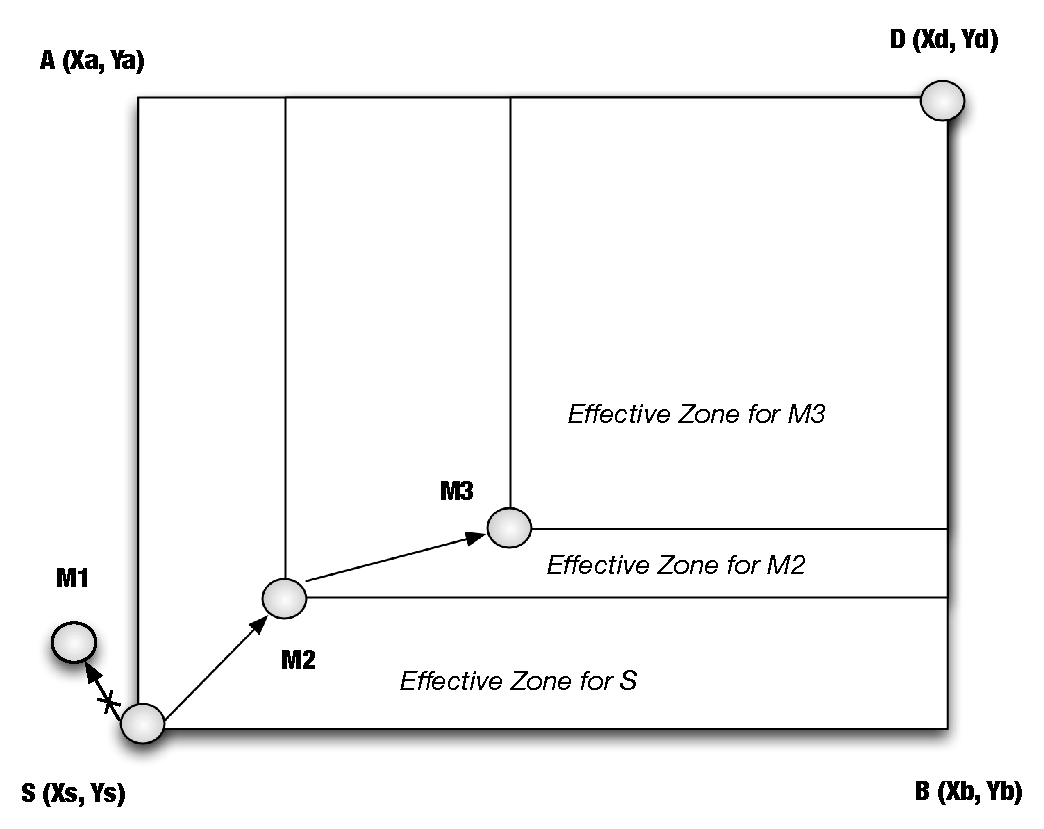
\includegraphics{adaptiveZone.eps}
\caption{Adaptive Effective Zone}
\end{figure}
As show in the figure 1, when a node M2 receives a message from sender S, it will calculate the effective zone(a rectangle ADBS) with the location of destination D and S. If one node that hears the message is in the zone, it will receive the message (in this case, the node is M2, and it will broadcast forward the message), otherwise it will discards the message (M1). After M3 receives message form M2, it will calculate effective zone again, so the zone is adaptive for different nodes.

\section*{2.1.1~~~~Data Structure}

The network layer only adds header and tailer to each payload, the source location and source ID is stored in the header and the tailer is saved for further using.\\[1em]

Since the location information can typically fit well into one packet, the end-to-end layer don't need to partition it, furthermore, some kind of ECC code is needed because the location information needs to be precise.\\[1em]

The image is pretty big compared to the packet size, so the partitioning is needed. It can tolerant fault in data transferring, so no ECC code even checksum is ignored for the sake of throughput. \\[1em]

To distinguish location information from image, we need to add some field in front of the message. The image message needs to add some more field after the distinguish data to specify to which image this message belongs and the ID of this message in the image. An ID of each message is also needed for further use, it can be generated by a timestamp function appending the unique device ID.\\[1em]

In further development, a mode modifier is needed for the sake that there is a message needed to be transferred urgently (a location information almost 5 minutes from sent), even more unexpected data fields is needed during development, so we save some fields here.\\[1em]

%message meta data: origin source time ok node list path node list id origin send time message content: image(optional) and origin source location information%

For each device, it should maintain the location information and the image of its own, a list of messages received is also needed to avoid unexpected resending the message. It can also maintain a local path cache to  accelerate later sending to some extent, the mechanism is specified later.\\[1em]

\section*{2.1.2~~~~Adaptive Effective Zone Algorithm}
In order to let messages reach the base station and maximize the throughput, we adopt a location based algorithm instead of brute force algorithm to broadcast messages.\\[1em]

The description mentioned below only focus on the whole process of routing and ignore the detail of other things such as reliability, security issues etc.\\[1em]

\begin{enumerate}
\item S invoke the predefined scan() function to get a list of tuples (node, loss\_prob), for the sake of improving effectivity, then S chooses those nodes whose loss\_prob is lower than P, and who is not in the origin path.
\item S broadcasts a message which has an unique ID to nearby nodes. The message contains the location information of S, a list which contains nodes chosen in Step1, the content information which contains location information of origin source node(here is S) or image information.
\item If node A receives the message sent by S, the first thing is to check whether the message has been sent from A, and discard it if it has. Then, check whether S wants A to broadcast the message by checking the node list. If not, discard it, too. 
\item Then A calculates whether A is in the effective zone calculated using the location information of the sender and the base station, if A is not in the effective zone, discard it. Otherwise it rebroadcast the content message along with updated mete data as S does and invokes receive().
\item If all things go well, after the  iterative processes of Step 1 to 5, the message will reach D. Then D responses with an overall ACK to the sender of the message to him for example, M2. M2 now knows he can pass the message and pass the ACK to his sender M1, now M1 knows he can pass the message to D via M2, so he adds M1 to cache, next time a message is received, he can send via M1, thus accelerate the sending of message.
\end{enumerate}

\section*{2.2~~~~Transfer Protocol}

Since image and location information differ in size and importance, we adopt different end-to-end protocols for them.

\section*{2.2.1~~~~Location Transfer Protocol}

Location information is the most important in the transfer system, so each time a location information is received from the satellite or other devices, it sends it towards the base immediately.\\[1em]

To make the location information be received to the base as soon as possible, each node broadcast the location message until it receives an ACK. When a message is received and correctly decoded, the node responses with an ACK to the sender.\\[1em]

We can make sure the transfer succeed by calling send() to the node cached first if it is not empty, and then broadcast the message.\\[1em]

At last, to reduce the overall pressure of the communication system, each node maintains a list of the messages received and decoded correctly. If the same message is received later, it can just response with an ACK and discard the message.\\[1em]

\section*{2.2.2~~~~Image Transfer Protocol}

Compared to the location information, images have the following characteristics:

\begin{itemize}
\item large
\item no strict requirement for correctness
\end{itemize}

%We adopt another approach to dealing with image information:
 
%\begin{enumerate}
%\item the sender partitions the image into several messages and push them into the image stack
%\item the sender sends each of the packet of image to only one nodes within the loss probability 
%\item if an ACK is received for this message, discard this message, otherwise, resends to other nodes
%\item if a node receives a message of type image, it responds with an ACK, puts this message into the stack, and goes on sending repeating the steps above.
%\end{enumerate}

We need to modify our protocol of important data transfer, we don't call send() this time to reduce pressure of these nodes and make bandwidth space for location information.\\[1em]

%Note that we send the message to just one node instead of all, this is done to reduce the pressure and make bandwidth space for location information.\\[1em]

\section*{2.3~~~~Handling of Extreme Circumstances}

Although the communication system works well following the simple algorithms and protocol above, some extreme circumstances need to be considered, thus makes the system more and more complicated, more and more fields are added, though we tried to make things as simple as possible.

\section*{2.3.1~~~~Basic Lost Handling}

In our location based algorithm, many nodes discard the packet for the sake of improving throughput. As a result, there will be a problem that S can not reach D through the nodes in the effective zone. Therefore, we need a basic mechanism to handle such problem along with the lost problem in send or receive process.\\[1em]

If the sender S does not receive confirm information from D for a while, it first rebroadcast the message for several times and then expand effective zone from rectangle into the all space.\\[1em]

\section*{2.3.2~~~~Burst Mode}

Since location information must be sent to base station within 5 minutes, burst mode is introduced to ensure this feature. Every location message holds  the origin send time. If intermediate nodes find that the time has passed for a long time such as 4.5 minutes, it will change into burst mode for this message which accelerate the frequency of rebroadcast and higher the priority of this message.

\section*{2.4~~~~Malicious Nodes Handling}

Nodes in the system should distinguish malicious nodes by some strange behavior, so we classify different kinds of malicious nodes and handle it separately.

\subsection*{Type One}
The malicious node hear a legitimate message, then broadcasts many copy(such as one million) of this message pretending it received it from the source.
\paragraph{How to handle}
We add a counter to every node. When a node receive abnormal number of messages of one sender, the node can mark sender as a malicious node and discard message from it. \\

In this situation, we effectively prevent the millions copies of message from propagating forward to the whole system. However, nodes around the malicious node will suffer millions of connections till the malicious node stop sending, so these nodes will lose the ability to receive other messages. The only thing we can do to handle this relative small problem is send warning message to the base station or the other people to handle the malicious node in physical way. 
\subsection*{Type TWO}
The malicious node X receives a message, responses to the sender but stop forward the message and the sender will consider X will do its job as usual. 
\paragraph{How to handle}
%Not holds this time since broadcast only gives the message to one (or more) node(s)
%Under most situation, it is not a big problem since other nodes around sender will do their job as usual.\\
We can know this if no ACK of location from base is sent back for a long time, thus we can send twice. If there is still no response, we can send several times, or we can mark those who have received the message as bad in cache, next time we can send according to the node list generated by scan().

However, when all valid nodes (in effective zone and low lost probability) around sender are malicious node, the sender can not send message to the base station. We will discuss it further in our report.%how to handle?
\subsection*{Type THREE}
The malicious node change the message and send forward to the base station. 
\paragraph{How to handle}
The method is easy to handle by encrypting the message, but how to implement it correctly and prevent malicious node from decrypting is a difficult theoretical problem and beyond our scope.

\section*{3~~~~Future Work}
The system ensures that locations of first responders reliably reach the base station within 5 minutes, while also maximizing the throughput of pictures back to the base station. We will consider more situations, optimize it further and analyze the system in different situation. \\[1em]

Word Count:1183(exclude title page)

\end{document}